\renewcommand{\thechapter}{\roman{chapter}}
\setcounter{chapter}{4}
\setcounter{figure}{0}

\unchapter{Préambule multimodalité}
\label{chap:preamble_multimodal}
Lors de la précédente partie consacrée à la \acrlong{rcm}, différentes méthodes sont proposées afin d'obtenir des prédictions au niveau des images et des lésions. Cette dernière partie va permettre de mettre au point et d'évaluer des stratégies permettant la mise en place de processus multimodaux d'aide au diagnostic des lésions malignes mais surtout des lésions de type \gls{lm} et \gls{lmm}. À cette fin, ce préambule présente lors des prochains paragraphes les données employées à cet effet et reprend les points important de l'étude clinique de référence.\par

Pour rappel, les données de photographie clinique et de dermatoscopie ont été mises de côté lors des expériences sur la \gls{rcm} menée lors de la \Cref{part:microscopy}. Ainsi, cette nouvelle partie intègre l'ensemble des données de lésions obtenues dans le cadre de l'étude de Cinotti et al.~\cite{Cinotti2018}, soit 223 lésions pour lesquelles sont mises à disposition les acquisitions issues des modalités de \textit{photographie clinique}, de \textit{dermatoscopie} et \gls{rcm}. Ces données sont focalisées majoritairement autour de lésions malignes de type \gls{lm} et de \gls{lmm} et lésions bénignes proches de ces deux pathologies, susceptibles d'induire le praticien en erreur.\par 

\begin{figure}[H]
    \begin{center}
        \includegraphics[width=\linewidth]{contents/iii_preamble_multimodal/resources/example_clinical_crop.pdf}
        \caption{Exemples de données de photographie clinique recadrées manuellement autour de la zone d'intérêt pour le besoin de ce manuscrit.}
        \label{fig:example_clinical_crop}
    \end{center} 
\end{figure}\par
\clearpage

De manière plus détaillée, chaque lésion issue de ce jeu de données comporte~:
\begin{itemize}
    \item des données de \textbf{photographie clinique}, \textit{une image par lésion}. Pour cinq de ces lésions, plusieurs images de photographie clinique étaient mises à disposition, \textbf{seule la plus pertinente d'entre elles a été conservée}. De plus, aucun protocole ne régit l'acquisition de ces images ce qui abouti à une grande diversité, dont la lésion représente parfois qu'une faible portion de celle-ci. Afin de limiter cette diversité, \textbf{ces images sont recadrées manuellement} pour l'objet de ce travail. La résolution spatiale de ces images recadrées est comprise entre 250 $\times$ 250 pixels pour les plus petites d'entre elles à plus de 2000 $\times$ 2000 pixels pour les plus conséquentes.
    \item des données de \textbf{dermatoscopie}, \textit{une image par lésion}. Ces images sont utilisées de manière brute, pour lesquelles aucun traitement n'a été jugée nécessaire. En effet, le principe de cette modalité permet d'obtenir des images assez homogène malgré l'absence de protocole d'acquisition. La résolution spatiale de ces images est comprise entre 480 $\times$ 640 pixels pour les plus petites d'entre elles à 3312 $\times$ 4416 pixels pour les plus conséquentes. Cependant, environ 85\% de ces lésions possèdent une résolution spatiale de 3312 $\times$ 4416 pixels.
    \item des données de \textbf{\gls{rcm}}, dont le nombre varie \textit{de quelques images à plusieurs centaines par lésion}. Pour chaque lésion, ces images sont sélectionnées par deux des trois médecins investigateurs de l'étude~\cite{Cinotti2018}. L'acquisition de ces données provient essentiellement de la \gls{dej}, particulièrement adapté à l'observation de ce phénomène. Ces données ont été plus longuement décrites lors du \Cref{chap:preamble_microscopy}.
\end{itemize}\par

À partir de ces éléments, les experts de cette étude ont obtenus les divers scores suivants~:
\begin{itemize}
    \item sur les données de \textbf{photographie clinique}, les 15 experts examinés ont obtenus une sensibilité de 0,72$\pm$0,08 et une spécificité de 0,78$\pm$0,08 sur l'ensemble des lésions malignes. Aucune information n'est mise à disposition sur les pathologies de \gls{lm} et \gls{lmm} sur cette modalité.
    \item sur les données de \textbf{dermatoscopie}, les 15 experts examinés ont obtenus une sensibilité de 0,69$\pm$0,10 et une spécificité de 0,85$\pm$0,06. Sur les pathologies de \gls{lm} et \gls{lmm}, ces scores s'écartent de manière significative avec une valeur de sensibilité de 0,61$\pm$0,15 et de spécificité de 0.92$\pm$0,05.
    \item sur les données de \textbf{\gls{rcm}}, les 12 experts examinés ont obtenus une sensibilité de 0,84$\pm$0,05 et une spécificité de 0,75$\pm$0,06. Sur les pathologies de \gls{lm} et \gls{lmm}, ces scores deviennent plus homogènes avec une valeur de sensibilité de 0,80$\pm$0,07 et de spécificité de 0.81$\pm$0,05.
\end{itemize}\par

En termes de courbes \gls{roc}, ces précédents résultats sont bien moins nuancés. Ces courbes rapportées au score \gls{auc}, les experts accomplissent sur la dermatoscopie un score de 0,85 contre 0,86 sur la \gls{rcm} sur l'ensemble des lésions malignes. Sur les lésions de type \gls{lm} et \gls{lmm}, les experts accomplissent sur la dermatoscopie et sur la \gls{rcm} un score de 0,88. Ces résultats de courbes \gls{roc} et de scores \gls{auc} sur la \Cref{fig:results_roc_experts}.\par

\begin{figure}[H]
    \begin{center}
        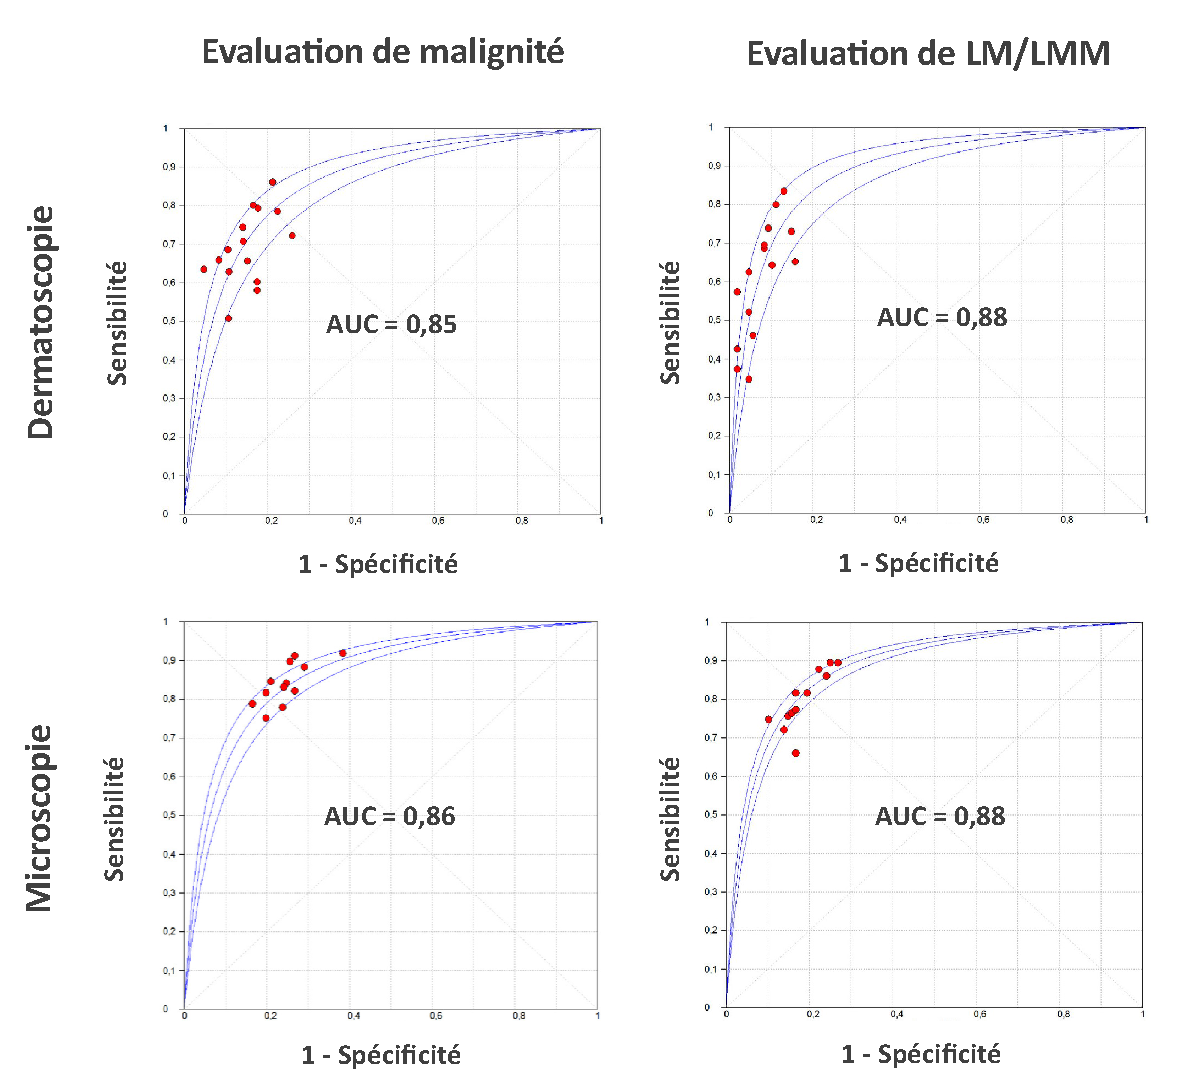
\includegraphics[width=\linewidth]{contents/iii_preamble_multimodal/resources/results_roc_experts.pdf}
        \caption{Courbes \gls{roc} issues de l'évaluation des données de dermatoscopie et de \gls{rcm} par les experts~\cite{Cinotti2018}. En haut, les résultat des 15 experts mené sur la modalité de dermatoscopie ; En bas, les résultat des 12 experts mené sur la modalité de \gls{rcm}. À gauche, les résultats sur la détection d'éléments malins ; À droite, le résultat des experts mené sur la détection de \gls{lm} et \gls{lmm}.}
        \label{fig:results_roc_experts}
    \end{center} 
\end{figure}\par

En revanche, cette étude ne met pas à disposition d'éléments relatifs à une prise en charge séquentielle et ne donne pas lieu à un objectif particulier contrairement à la précédente partie. Néanmoins, l'objectif visé dans cette partie sans quantification exacte est d'optimiser ce processus clinique tout en limitant la dégradation des performances. À nouveau, les méta-données issues des informations patient ne sont pas exploitées seules les données images sont employés dans la mise en place de ce processus. Pour les mêmes raisons que précédemment, ces méta-données ne sont pas représentatives de la population réelle, et peuvent de ce fait introduire un biais au sein des méthodes présentées par l'apport de corrélations invalides dans le monde réel.\par

Afin de répondre à ces objectifs et de clore l'objet de ce manuscrit, cette partie dédiée à la multimodalité propose diverses approches en cascades susceptibles de convenir à des applications en milieu clinique. Ainsi, ces éléments sont étudiées au sein du \Cref{chap:chapter_8}, par l'étude de processus de décision séquentiel d'aide au diagnostic clinique.\par
